\documentclass{llncs}

\usepackage[utf8]{inputenc}
\usepackage{hyperref}
\usepackage{times}
\usepackage[T1]{fontenc}
\usepackage{listings}
\usepackage{graphicx}
\usepackage{multicol}
\usepackage{geometry}

\lstset{language=C, frame=tlrb,basicstyle=\scriptsize,breaklines=true}

\begin{document}

\bibliographystyle{splncs}

\title{Implementing BLAS SSPR}
\author{Andrés More\inst{1} \inst{2}}

\institute{Intel Software Argentina (Argentina Software Design Center) \\
\email{andres.more@intel.com} \\ 
\and
Instituto Aeronáutico Córdoba \\
\email{amore@iua.edu.ar}}

\maketitle

\begin{abstract}

This work reviews the experience of implement different versions of the SSPR rank-1 update operation
of the BLAS library. The main objective was to contrast CPU versus GPU usage,
not only considering performance but also programming effort and complexity.
This work contributes with a sample procedure to analyze BLAS kernel implementations in CPU and GPU,
how to start using GPU libraries and offloading, how to analyze their performance and
the issues faced and how they were solved.

\keywords{GPGPU, BLAS, SSPR, CUDA}
\end{abstract}

\section{Introduction}

With the growth of GPGPU there will be lots of people trying to implement a math kernel operation both in CPU
and GPU, optimize and do a performance comparison to double check if performance gains are relevant or not.

\subsection{SSPR}

The operation computes a rank-1 update of a simmetric matrix of single precision floating point numbers.

SSPR performs the symmetric rank 1 operation show in Equation \ref{eq:math},
where $ \alpha $ is a real scalar, $ x $ is an $ n $ element vector and $ A $ is an
$ n $ by $ n $ symmetric matrix, supplied in packed form.
A graphical representation of the operation is shown in Figure \ref{fig:math}.

\begin{equation}
    A := \alpha \times x \times x ^{T} + A
\label{eq:math}
\end{equation}

\begin{figure}
\begin{center}
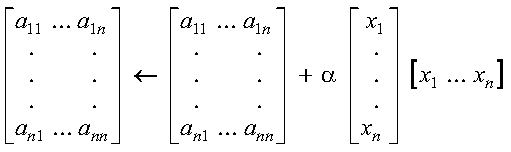
\includegraphics[scale=0.7]{math.png}
\caption{Graphical representation of rank 1-update}
\label{fig:math}
\end{center}
\end{figure}

The operation belongs to level 2 BLAS (Basic Linear Algebra Subprograms) \cite{blas} \cite{blas-updated},
as it runs over a matrix-vector combination. Matrix vector multiplication as $ O(N^{2}) $ complexity.\cite{matmul}.

However, the matrix is required to be represented as a vector
which contains only half of the symattric matrix triangular, packed sequencially per column.

Represented by Equation \ref{eq:packed}. In particular, the vector has a size of $ (n \times (n + 1) / 2) $.

\begin{equation}
AP(i + ( j \times (j-1) / 2) = A _{ij} (\forall j \geq i)
\label{eq:packed}
\end{equation}

Operation signature in FORTRAN is defined as

\begin{lstlisting}[caption={SSPR Fortran Signature},label={lst:signature}]
SUBROUTINE SSPR(UPLO,N,ALPHA,X,INCX,AP)
          .. Scalar Arguments ..
          REAL ALPHA
          INTEGER INCX,N
          CHARACTER UPLO
          ..
          .. Array Arguments ..
          REAL AP(*),X(*)
\end{lstlisting}

Arguments.

\begin{tabular} {|l|l|} \hline
UPLO & specifies whereas upper/lower triangular part of A is supplied in array \\ \hline
N & specifies the order of the matrix A \\ \hline
ALPHA & specifies the scalar alpha \\ \hline
X & array of dimension at least $ ( 1 + ( n - 1 ) * abs( INCX ) ) $ \\ \hline
INCX & specifies the increment for the elements of X \\ \hline
AP & array of dimension at least $ ( ( n*( n + 1 ) ) / 2 ) $ \\ \hline
\end{tabular}

\subsection{Testbed}

The system used for tests was a HP Mobile Workstation EliteBook 8530w having integrated
an Intel CPU model T9600 \footnote{\href{http://ark.intel.com/products/35563}{CPU specifications}}
plus a Quadro FX 770m GPU \footnote{\href{http://www.nvidia.com/docs/IO/57883/PO\_Quadro\_FAM\_Mar08\_FINAL\_LowRes.pdf}{GPU specifications}}.

\begin{verbatim}
cpu family: 6
model: 23
model name: Intel(R) Core(TM)2 Duo CPU T9600 @ 2.80GHz
stepping: 10
cpu MHz: 2793
cache size: 6144 KB
fpu: yes
cpuid level: 13
flags: fpu vme de pse tsc msr pae mce cx8 apic sep mtrr
pge mca cmov pat pse36 clflush dts acpi mmx fxsr sse sse2
ss ht tm pbe pni dtes64 monitor ds_cpl vmx smx est tm2
ssse3 cx16 xtpr pdcm sse4_1 xsave osxsave lahf_lm
TLB size: 0 4K pages
\end{verbatim}

CUDA Toolkit version 4.2 was used, published in February 2012.
The GPU card cames with 512MB of memory, meaning that in average during executions
there is about 462 MB of global memory available for computation.

\begin{verbatim}
capabilities.name = Quadro FX 770M
capabilities.totalGlobalMem = 512.00 MB
capabilities.sharedMemPerBlock = 16.00 KB
capabilities.regsPerBlock = 8192
capabilities.warpSize = 32
capabilities.memPitch = 2097152.00 KB
capabilities.maxThreadsPerBlock = 512
capabilities.maxThreadsDim = 512 512 64
capabilities.maxGridSize = 65535 65535 1
capabilities.totalConstMem = 64.00 KB
capabilities.major = 1
capabilities.minor = 1
capabilities.clockRate = 1220.70 MHz
capabilities.textureAlignment = 256
capabilities.deviceOverlap = 1
capabilities.multiProcessorCount = 4
cudaMemGetInfo.free = 462 MB
\end{verbatim}

\subsection{CUDA Programming}

Model?

Library? 

\section{Algorithms}

As part of the work 4 different versions of SPRR functions were implemented.

In order to streamline analysis only support for upper matrices with 1 increments were implemented.

\subsection{CPU Sequential}

Using both the original BLAS implementation \footnote{\href{http://www.netlib.org/blas/sspr.f}{BLAS SSPR implementation.}} and the GNU Scientific Library version \footnote{\href{gsl/blas/source\_spr.h}{GSL SSPR implementation.}} an initial CPU sequential version was implemented. 

It is used as baseline for future comparisons. This relies on the packed matrix representation using a plain array.
A naive implementation of the mathematical definition was not used as proper speedup computation requires best known sequential algorithm \cite{debunking}.

\begin{lstlisting}[caption={Naive SSPR CPU Implementation},label={lst:naive}]
for (j=0;j<n;j++)
	for(i=0;i<=j;i++) {
		ap[k] += alpha*x[i]*x[j];
		k++;
}
\end{lstlisting}

\begin{lstlisting}[caption={Optimized SSPR CPU Implementation},label={lst:cpuopt}]
for (i = 0; i < n; i++) {
	const float tmp = alpha * x[i];

	for (j = 0; j <= i; j++)
		ap[((i * (i+1)) / 2+j )] += x[j] * tmp;
}
\end{lstlisting}

Here we can estimate that the required computation per data quantity is not enough to justify accelarator offload time.
It is expected then that a GPU version of it is not going to have huge performance increments for small data.

\subsection{GPU cuBLAS}

Nvidia CUDA \cite{cuda} provides its own version of BLAS rountines, which are heavily optimized to their architecture. Using cuBLAS \cite{cublas} library requires one call.

This highly optimized code can be found in the package available to registered developers,
inside {\tt sspr.cu} and {\tt sspr.h} files. The main routine is {\tt cublasSspr()}.

\begin{lstlisting}[caption={cuBLAS SSPR GPU Implementation}, label={lst:gpucublas}]
ret = cublasSspr(handle, mode, n, &alpha, cx, incx, cap);
if (ret != CUBLAS_STATUS_SUCCESS)
	err("cublasSspr: %d (%s)", ret, cublas2str[ret]);
\end{lstlisting}

This implementation first loads into device shared memory elements reused during computation, then computes several matrix elements for hardware thread. It also uses cheap bit shifting instead of expensive division by 2 to locate elements inside the packed matrix.

To use support function as explicitly recomended you need to rely on utilities like:

\begin{itemize}
\item {\tt cublasCreate()}, 
\item {\tt cublasSetVector()}
\item {\tt cublasGetVector()}
\item {\tt cublasDestroy()};
\end{itemize}

including error handling with opaque datatypes like:

\begin{itemize}
\item {\tt cudaError\_t}
\item {\tt cublasHandle\_t}
\item {\tt cublasStatus\_t}
\item {\tt cublasFillMode\_t}
\end{itemize}

\subsection{GPU Naive}

A direct translation to GPU using just one thread per X element, computing the result in parallel.

\begin{lstlisting}[caption={Naive SSPR GPU Implementation},label={lst:gpunaive}]
__global__ void sspr_naive_kernel(int uplo, int n, float alpha, const float *x, int incx, float *ap) {
	int i = blockIdx.x * blockDim.x + threadIdx.x;
	if (i < n) {
		const float tmp = alpha * x[i];
		int j = 0;
		for (j = 0; j <= i; j++)
			ap[((i*(i+1))/ 2 + j)] += x[j] * tmp;
	}
}
\end{lstlisting}

To execute the kernel

\begin{lstlisting}
sspr_naive_kernel<<< (n / capabilities.maxThreadsPerBlock), (capabilities.maxThreadsPerBlock) >>>(uplo, n, alpha, cx, incx, cap);
\end{lstlisting}

\subsection{GPU using shared-memory}

An initial optimization using shared memory to reduce access time to the X vector.
Every thread on the same thread block loads in shared memory one element in parallel.
During computation elements are gathered from shared or global memory.

\begin{lstlisting}[caption={Optimized SSPR GPU Implementation},label={lst:gpuoptimized}]
__global__ void sspr_optimized_kernel(int uplo, int n, float alpha, const float *x, int incx, float *ap) {
	int i = blockIdx.x * blockDim.x + threadIdx.x;
	if (i < n) {
		int tid = threadIdx.x;
		extern __shared__ float cache[];
		float *xi = (float *) cache;
		xi[tid] = x[i];
		__syncthreads();
		const float tmp = alpha * x[i];
		int j = 0;
		for (j = 0; j <= i; j++) {
			if (blockIdx.x * blockDim.x < j &&	blockIdx.x * blockDim.x + 1 > j)
				ap[((i*(i+1))/ 2 + j)] += xi[j] * tmp;
			else
				ap[((i*(i+1))/ 2 + j)] += x[j] * tmp;
		}
	}
}
\end{lstlisting}

\section{Results}

Figure \ref{fig:speedup} shows wall clock times in seconds with varying matrix sizes.
Times are geometric mean of 32 executions in order to reduce measurement noise.
To validate results the output matrix was reduced to a single figure being the common global sum of the elements.

\begin{figure}
\begin{center}
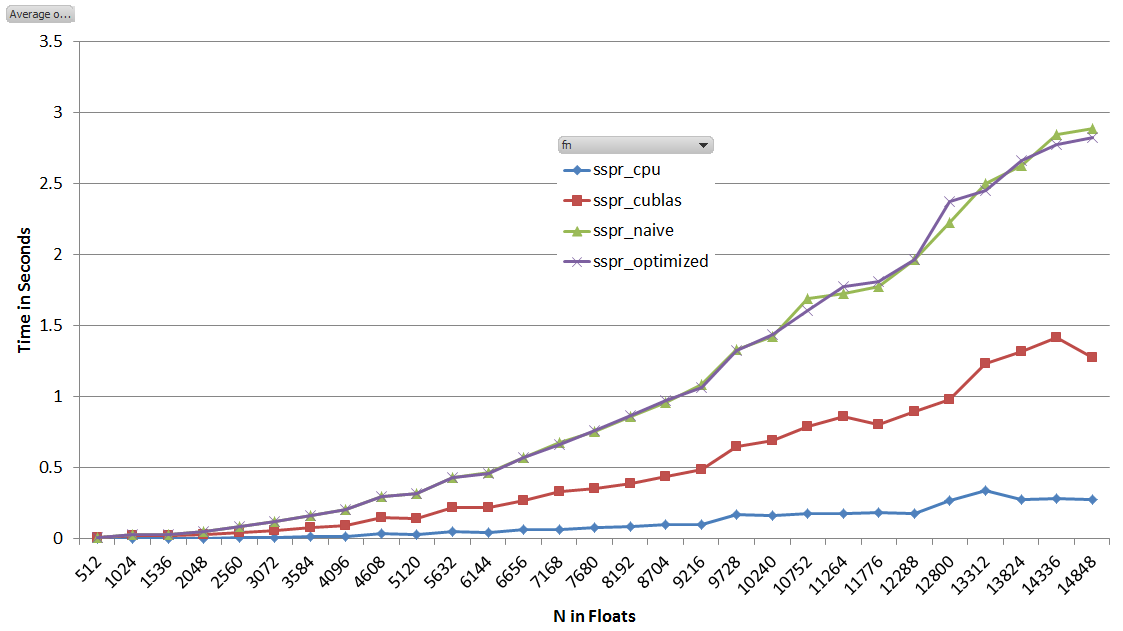
\includegraphics[scale=0.7]{speedup.png}
\caption{speedup}
\label{fig:speedup}
\end{center}
\end{figure}

Here we can clearly see that the introduced shared memory optimization do not positively impact execution time,
so cuBLAS strategy is hence superior. However, the CPU sequential and optimized version is still better.

\section{Performance Analysis}

\subsection{GPU Registers}

CUDA {\tt nvcc} compiler can be configured to show extra information about the number of registers used during execution. With this you can check that the register usage is minimal or according to your needs.

\begin{verbatim}
ptxas info: Compiling entry function 'sspr\_naive\_kernel' for 'sm\_13'
ptxas info: Used 7 registers, 48+16 bytes smem, 4 bytes cmem[1]
ptxas info: Compiling entry function 'sspr\_optimized\_kernel' for 'sm\_13'
ptxas info: Used 10 registers, 48+16 bytes smem, 4 bytes cmem[1]
\end{verbatim}

It was discovered that running with {\tt --arch=compute\_11} did not included this output,
but using {\tt -arch=sm\_13} instead solved the issue. 
The first one uses the compute capability version, the second the hardware architecture generation.

\subsection{Nvidia Visual Profiler}

The {\tt nvvp} tool inside the GPU depicts a visual execution profile, useful when trying to optimize.
On this case the tool identified:

\begin{itemize}
\item there is no overlap between data transfer and computation
\item the data transfer action does not fully saturate the available bandwidth
\item the computation does not fully load the available processing cores
\end{itemize}

This issues are caused by the nature of the problem and the device capabilities.
The device does not have enough internal memory to run an interesting enough problem,
and the required computation per transfered bytes does not justify GPU offloading with the current design.

\begin{figure}
\begin{center}
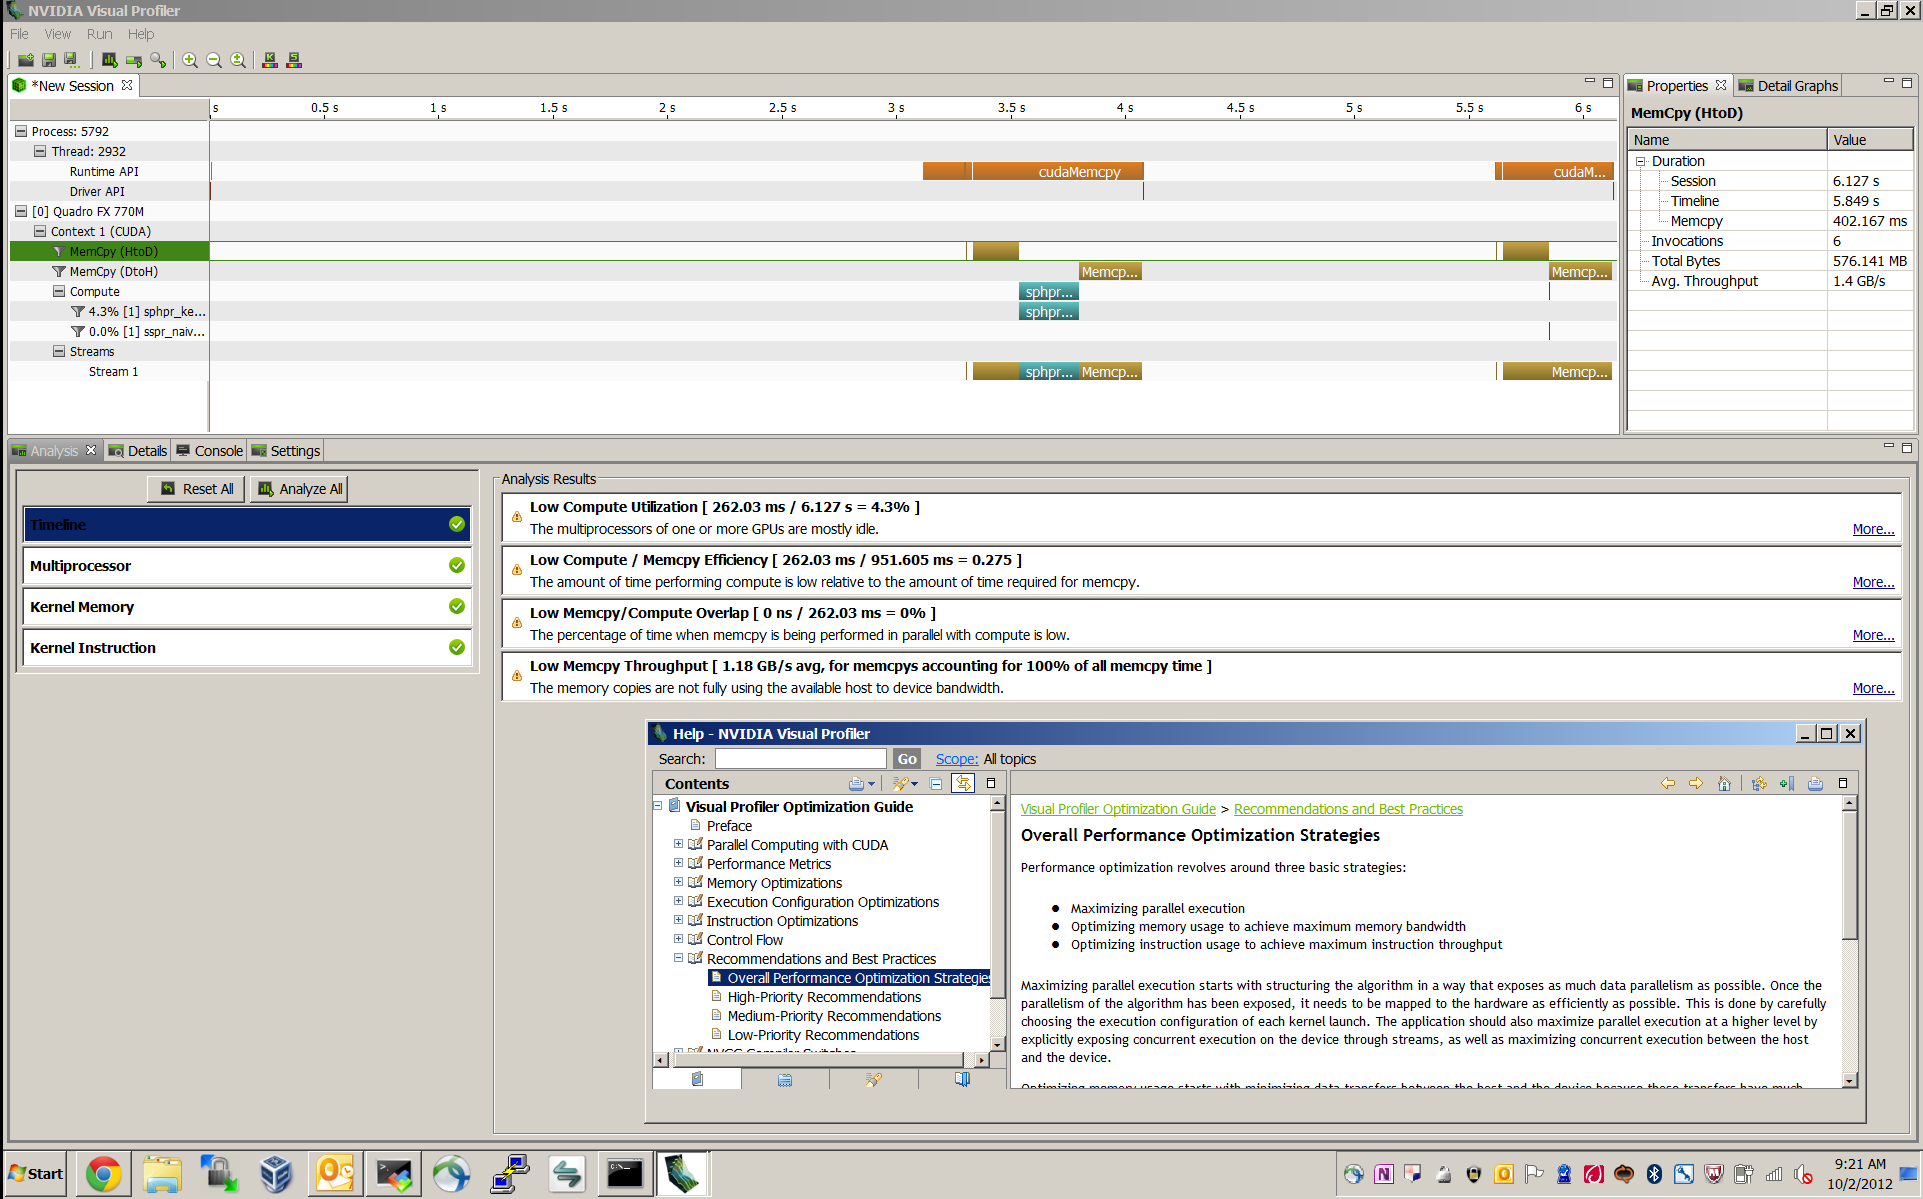
\includegraphics[width=\textwidth]{profiler.png}
\caption{Profiler}
\label{fig:profiler}
\end{center}
\end{figure}

\section{Speedups}

To measure speedup the input size was selected to fit inside most available memory in GPU.

\begin{verbatim}
SSPR_N = 14848 floats (packed 110238976 floats)
SSPR_ALPHA = 3.141593
memory = 420 MB
cudaMemGetInfo.free = 462 MB
\end{verbatim}

Most interesting speedup comparisons are shown in Table \ref{table:speedup}.

\begin{table}
\begin{center}
\begin{tabular} {|l|l|l|} \hline
cublas (1.4995 seg) & cpu (0.389625 seg) & 3.85x \\ \hline
naive (3.090625 seg) & cpu (0.389625 seg) & 7.93x \\ \hline
optimized (2.97325 seg) & cpu (0.389625 seg) & 7.63x \\ \hline
naive (3.090625 seg) & cublas (1.4995 seg) & 2.06x \\ \hline
optimized (2.97325 seg) & cublas (1.4995 seg) & 1.98x \\ \hline
optimized (2.97325 seg) & naive (3.090625 seg) & 0.95x \\ \hline
\label{table:speedup}
\end{tabular}
\end{center}
\caption{Speedup}
\end{table}

\subsection{Related Work}

Un estudio relacionado fue realizado por Microsoft Research \cite{ms-gaxpy}, comparando el rendimiento de BLAS nivel 2 en FPGA,
CPU y GPU. 
La gura 4 muestra los resultados que convalidan los obtenidos durante este trabajo. 
Es decir, la cantidad de computo no es signicante como para justicar la transferencia de datos.

\begin{figure}
\begin{center}
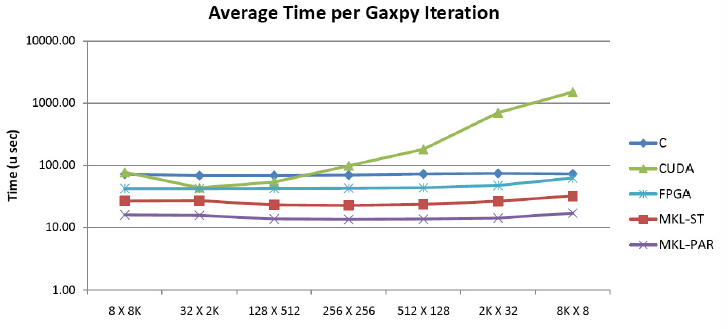
\includegraphics[width=\textwidth]{gaxpy.png}
\caption{Gaxpy: (reproduced from study)}
\label{fig:gaxpy}
\end{center}
\end{figure}

\section{Conclusions}

\subsection{cuBLAS}

The {\it cuBLAS} library does not provide a single call that take charge of the complete cycle:
initialization, data transference to accelerator, computation, data transference back to host.
Using low level primitives plus the error checking it is requried nearly 60 lines of code to run a BLAS routine.

{\it cuBLAS} lack an error formatter function to traduce error codes to human representations (similar to {\tt strerr()}). Some utility calls like {\tt cudaAlloc()} are deprecated but still referenced by sspr() and others.

In order to support both {\it Linux} and {\it Windows} environments small things need to be considered. 
Time keeping routines are not portable so a {\tt gettimeofday()} stub was coded.

\section{Future Work}

Other optimizations that require design changes (overlapping), or newer GPU architectures (zero-copy).
A good starting point is \href{http://docs.nvidia.com/cuda/cuda-c-best-practices-guide/}{CUDA C Best Practices Guide}.

\section*{Acknowledgements}

Reviewers, colleges.

\paragraph{Notes and Comments.}
Contact the author to get the sample code and any relevant guidance regarding how to approach a similar task.

\bibliography{sspr}

\appendix
\section{Reference Implementation}

\subsection{Makefile}

The Makefile used to automate the building process is shown below.

\lstinputlisting{Makefile.txt}

\subsection{Code}

The actual code is shown below.

\newgeometry{left=1cm, right=1cm}
\begin{multicols}{2}
\lstinputlisting[basicstyle=\tiny]{sspr.cu}
\restoregeometry
\end{multicols}

\end{document}
